
\section{Transient Performance of Two-Machine Geometric Lines}
\noindent In this Section we also use two part to introduce the two-machine model. It is the most significant difference between two-machine model and individual machine model that there is a buffer between two mahines. This will lead to a performance improvement and other complicated situation.

\subsection{Mathematical Dirivation of two-machine Model}
\label{mathematical two machine}
\noindent Suppose that we have a two-machine geometric line restrained by assumptions 1-8. shown in Figure \ref{State transition diagram of two geometric machine with buffer}. From the figure we can easily tell that the system obersve an ergodic Markov chain. Moreover, to machine state $s_i(n)$, we use $j(n)$ to imply the number of products in the buffer at the start of time slot $n$. Then, the state of the Markov chain can be described by a triple $(j(n),s_1(n),s_2(n))$, where $j(n)\in {0,1,...,N}$ and $s_1(n),s_2(n) \in {0,1}$. Apparently, the system will in total have states of $4(N+1)$.In order derive the transition probabilities from these states, we organize the states in the following form: we use $r(j,s1,s2)$ indicate the state number of the Markov chain state $(j,s_1,s_2)$, $h\in {0,1,...,N}, s_1,s_2\in {0,1}$. Given
\begin{equation}
	r(j,s_1,s_2) = 4j + 2s_1 +s_2 +1 .
	\label{definition of r}
\end{equation}
\begin{figure}[!h]
	\centering
	\includegraphics[]{figures/model_of_two_machine_with_buffer.tikz}
	\caption{State transition diagram of two geometric machine with buffer}
	\label{State transition diagram of two geometric machine with buffer}
\end{figure}
Then, the sequence of the $4(N+1)$ system states can be described in Table \ref{two machine state}. Moreover, we use a unique number from $1$ to $4(N+1)$ to represent each system state. For instance, State $1$ represents that both machines are broken down and the buffer is empty, while State $4(N+1)$ represents that both machines are working properly and the buffer is full. Furthermore, suppose a state number $r$, its related buffer and machines states can be described as follows:
\begin{equation}
	\begin{aligned}
		j^{(r)} =& \lf{\frac{r-1}{4}}\rf, s_1^{(r)} = \lf{\frac{r-1-4j^{(r)}}{2}}\rf \\
		s_2^{(r)} =& \lf{\frac{r-1-4j^{(r)-2s_1^{(r)}}}{1}}\rf
	\end{aligned}
\end{equation}
where $\lf{a}\rf$ refers to the largest integer not greater than $a$.
\begin{table}[H]
	\centering
	\caption{Arrangement of the System States $k = 0,1,...,N$}
	\begin{tabular}{c|llll}\hline
		State number$(r)$&$4k+1$ & $4k+2$  & $4k+3$ &  $4k+4$   \\\hline
		$j$   & $k$          & $k$      & $k$   &  $k$   \\
		$s_1$ & $0$          & $0$      & $1$   &  $1$ \\
		$s_2$ & $0$          & $1$      & $0$   &  $1$  \\ \hline
	\end{tabular}
	\label{two machine state}
\end{table}
Notice that the transition of $j(n)$ is deterministic defined by $s_1(n)$ and $s_2(n)$. For a given serial production lines, the equations that characterize the dynamics of $j(n)$ have been formulated in \cite{zhang2013transient}
\begin{equation}
	j(n+1)=j'(n) + s_1(n)min\{N-j'(n),1\}
	\label{number in buffer}
\end{equation}
where
\begin{equation}
	j'(n)=j(n)-s_2(n)min\{j(n),1\}
\label{occupation of buffer}
\end{equation}
In the above equtions, $j'(n)$ refers to the occupancy of the buffer as long as machine $m_2$ takes a part from the buffer at the start of time slot $n$.

The transitions of $s_i(n)$'s, meanwhile, are probabilistic based on \ref{transition probabilities}. Thus, we can view each of the $4(N+1)$ states, then, coming from \ref{number in buffer} and \ref{occupation of buffer}, distinguish all possible aimed states after one time slot by enumerating all four combining ways of $s_1(n)$ and $s_2(n)$, and, in the end, measure the corresponding transition probabilities using \ref{transition probabilities}. Suppose that we use $A_2$ to characterize the transition probability matrix derived and use $x_i(n)$, $i\in {1,2,...,4(N+1)}$, describe the probability that the system, in other words, the Markov chain, is in state $i$ in the period of the time slot $n$. Furthermore, the evolution of the system state, $x(n)=[x_1(n)x_2(n)...x_4(N+1)^{(n)}]^T$, is derived by
\begin{equation}
	x(n+1) = A_2x(n), \sum_{i=1}^{4(N+1)} x_i(n) = 1 .
\end{equation}
According the state arrangement \ref{definition of r}, we have
\begin{equation}
	\begin{aligned}
		x_{4j+1}(n)=&\text{Prob[$m_1$ down, $m_2$ down, buffer $b$ has $j$ parts at time $n$]}  \\
		x_{4j+2}(n)=&\text{Prob[$m_1$ down, $m_2$ up, buffer $b$ has $j$ parts at time $n$]}  \\
		x_{4j+3}(n)=&\text{Prob[$m_1$ up, $m_2$ down, buffer $b$ has $j$ parts at time $n$]} \\
		x_{4j+4}(n)=&\text{Prob[$m_1$ up, $m_2$ up, buffer $b$ has $j$ parts at time $n$]}.
	\end{aligned}
\end{equation}
Thus, according to the definitions derived in \ref{performance measures}, we can compute the performance measures of the two-machine geometric line system in the following way:
\begin{equation}
	\begin{aligned}
		PR(n)=&\  \text{Prob[$m_2$ up,buffer $b$ not empty during time $n$] }\\
		=&\ C_1x(n)=[C_{1,0}\ C_{1,1}\ ...\ C_{1,N}]x(n) \\
		CR(n)=&\ \text{Prob[m1 up and not blocked during time n]} \\
		=&\ C_2x(n)=[C_{2,0}\ C_{2,1}\ ...\ C_{2,N}]x(n)\\
		WIP(n)=&\ \sum_{i=1}^N i \cdot \text{Prob[buffer $b$ has $i$ parts at time $n$]} \\
		=&\ C_3x(n)=[C_{3,0}\ C_{3,1}\ ...\ C_{3,N}]x(n) \\
		ST_2=&\ \text{Prob[$m_2$ up and buffer $b$ empty at time $n$]} \\
		=&\ C_4x(n)=[C_{4,0}\ C_{4,1}\ ...\ C_{4,N}]x(n) \\
		BL_1=&\ \text{Prob[$m_1$ up, $m_2$ down,buffer $b$ is full at time $n$]} \\
		=&\  C_5x(n)=[C_{5,0}\ C_{5,1}\ ...\ C_{5,N}]x(n)
	\end{aligned}
\end{equation}
where
\begin{equation}
    \begin{aligned}
        C_{1,0}\ &= \ [0 0 0 0],  &C_{1,i}&= [0 1 0 1],  &i&= 1,...,N \\
        C_{2,N}\ &=\ [0 0 0 1],  &C_{2,i}&= [0 0 1 1],  &i&= 0,..,N-1 \\
        C_{3,i}\ &=\ [i i i i],  &i&=  0,...,N \\
        C_{4,0}\ &=\ [0 1 0 1],  &C_{4,i}&= [0 0 0 0],  &i&= 1,...,N  \\
        C_{5,N}\ &=\ [0 0 1 0],  &C_{5,i}&= [0 0 0 0],  &i&= 0,...,N-1
    \end{aligned}
\end{equation}
In consequence, all these performance measures can be described as linear related in system state $x(n)$.

As an example, suppose a two-machine geometric line given by ssumptions 1-8. with machine and buffer parameters
\begin{displaymath}
	P_1=0.03, R_1=0.18, P_2=0.06, R_2=0.21, N=10.
\end{displaymath}
Presume that both machines are initially broken and the buffer in the middle is initially empty. The Figure \ref{Transients of a two-machine geometric line} presents transients of the performance measures of this system. For both machines are initially down and the buffer is empty, $PR(n)$,$ CR(n)$ and $WIP(n)$ all rise from $0$. Moreover, $PR(n)$ and $CR(n)$ have significant difference during the transient process, while with $n$ growing larger, both converge to the same value because of the conservation of flow in steady state. In addition, for the buffer is empty in the beginning, $BL_1(n)$ stays zero (in other words, machine $m_1$ is not in blockage state) until $n > N$.

\begin{figure*}[!h]
	\centering
	\subfigure[]{
		\includegraphics[width=0.45\linewidth,height=0.35\linewidth]{figures/two_machine_pr_and_cr.tikz}
		\label{two machine pr and cr}}
	\subfigure[]{
		\includegraphics[width=0.45\linewidth,height=0.35\linewidth]{figures/two_machine_wip.tikz}	
		 \label{two machine wip}}
	\subfigure[]{
		\includegraphics[width=0.45\linewidth,height=0.35\linewidth]{figures/two_machine_bl_and_st.tikz}	
		\label{two machine bl and st}}
	\caption{Transients of a two-machine geometric line. (a) $PR(n)\ and\ CR(n)$;(b) $WIP(n)$; (c) $ST_2(n)\ and\ BL_2(n)$}
	\label{Transients of a two-machine geometric line}
\end{figure*}


\subsection{Implementation of two-machine model}
\label{c}
\noindent In the python platform, we still keep the \pythoninline{class Individual} and have a slight adjust to simulate a machine instance. The main modification is to add two instance to represent the buffer upstream and downstream respectively. Moreover, it also hold a flag to judge whether the machine is blocked or starved according to the state of buffer in up- and downstream so that it cannot process a part in a time slot. Meanwhile, we add another \pythoninline{class Buffer} to represent the buffer in the middle of two machines. The buffer have its own storage to denote the numbers of products it hold and the maximal capacity. In addition, it also implements the products receiving and taking away function by two method \pythoninline{add_one() } and \pythoninline{take_one()}.

We use an UML diagram (Figure \ref{two machine uml}) to describe the relationship between three class. The program procedure is as follow: first, in the script ''sim2.py'' create we a certain amount of production lines, and each contains an instance from \pythoninline{class TwoMachine}. Meanwhile, the \pythoninline{class TwoMachine} consists of two instances from \pythoninline{class Individual} which represent the first and second machine respectively, and a buffer instance from \pythoninline{class Buffer}. In addition, the function \pythoninline{one_slot()} simulate a process in one time slot, and then give the critical transient performance measures back  to script ''sim2.py'' in order that the data can be record in the file.

\begin{figure*}[!h]
	\centering
	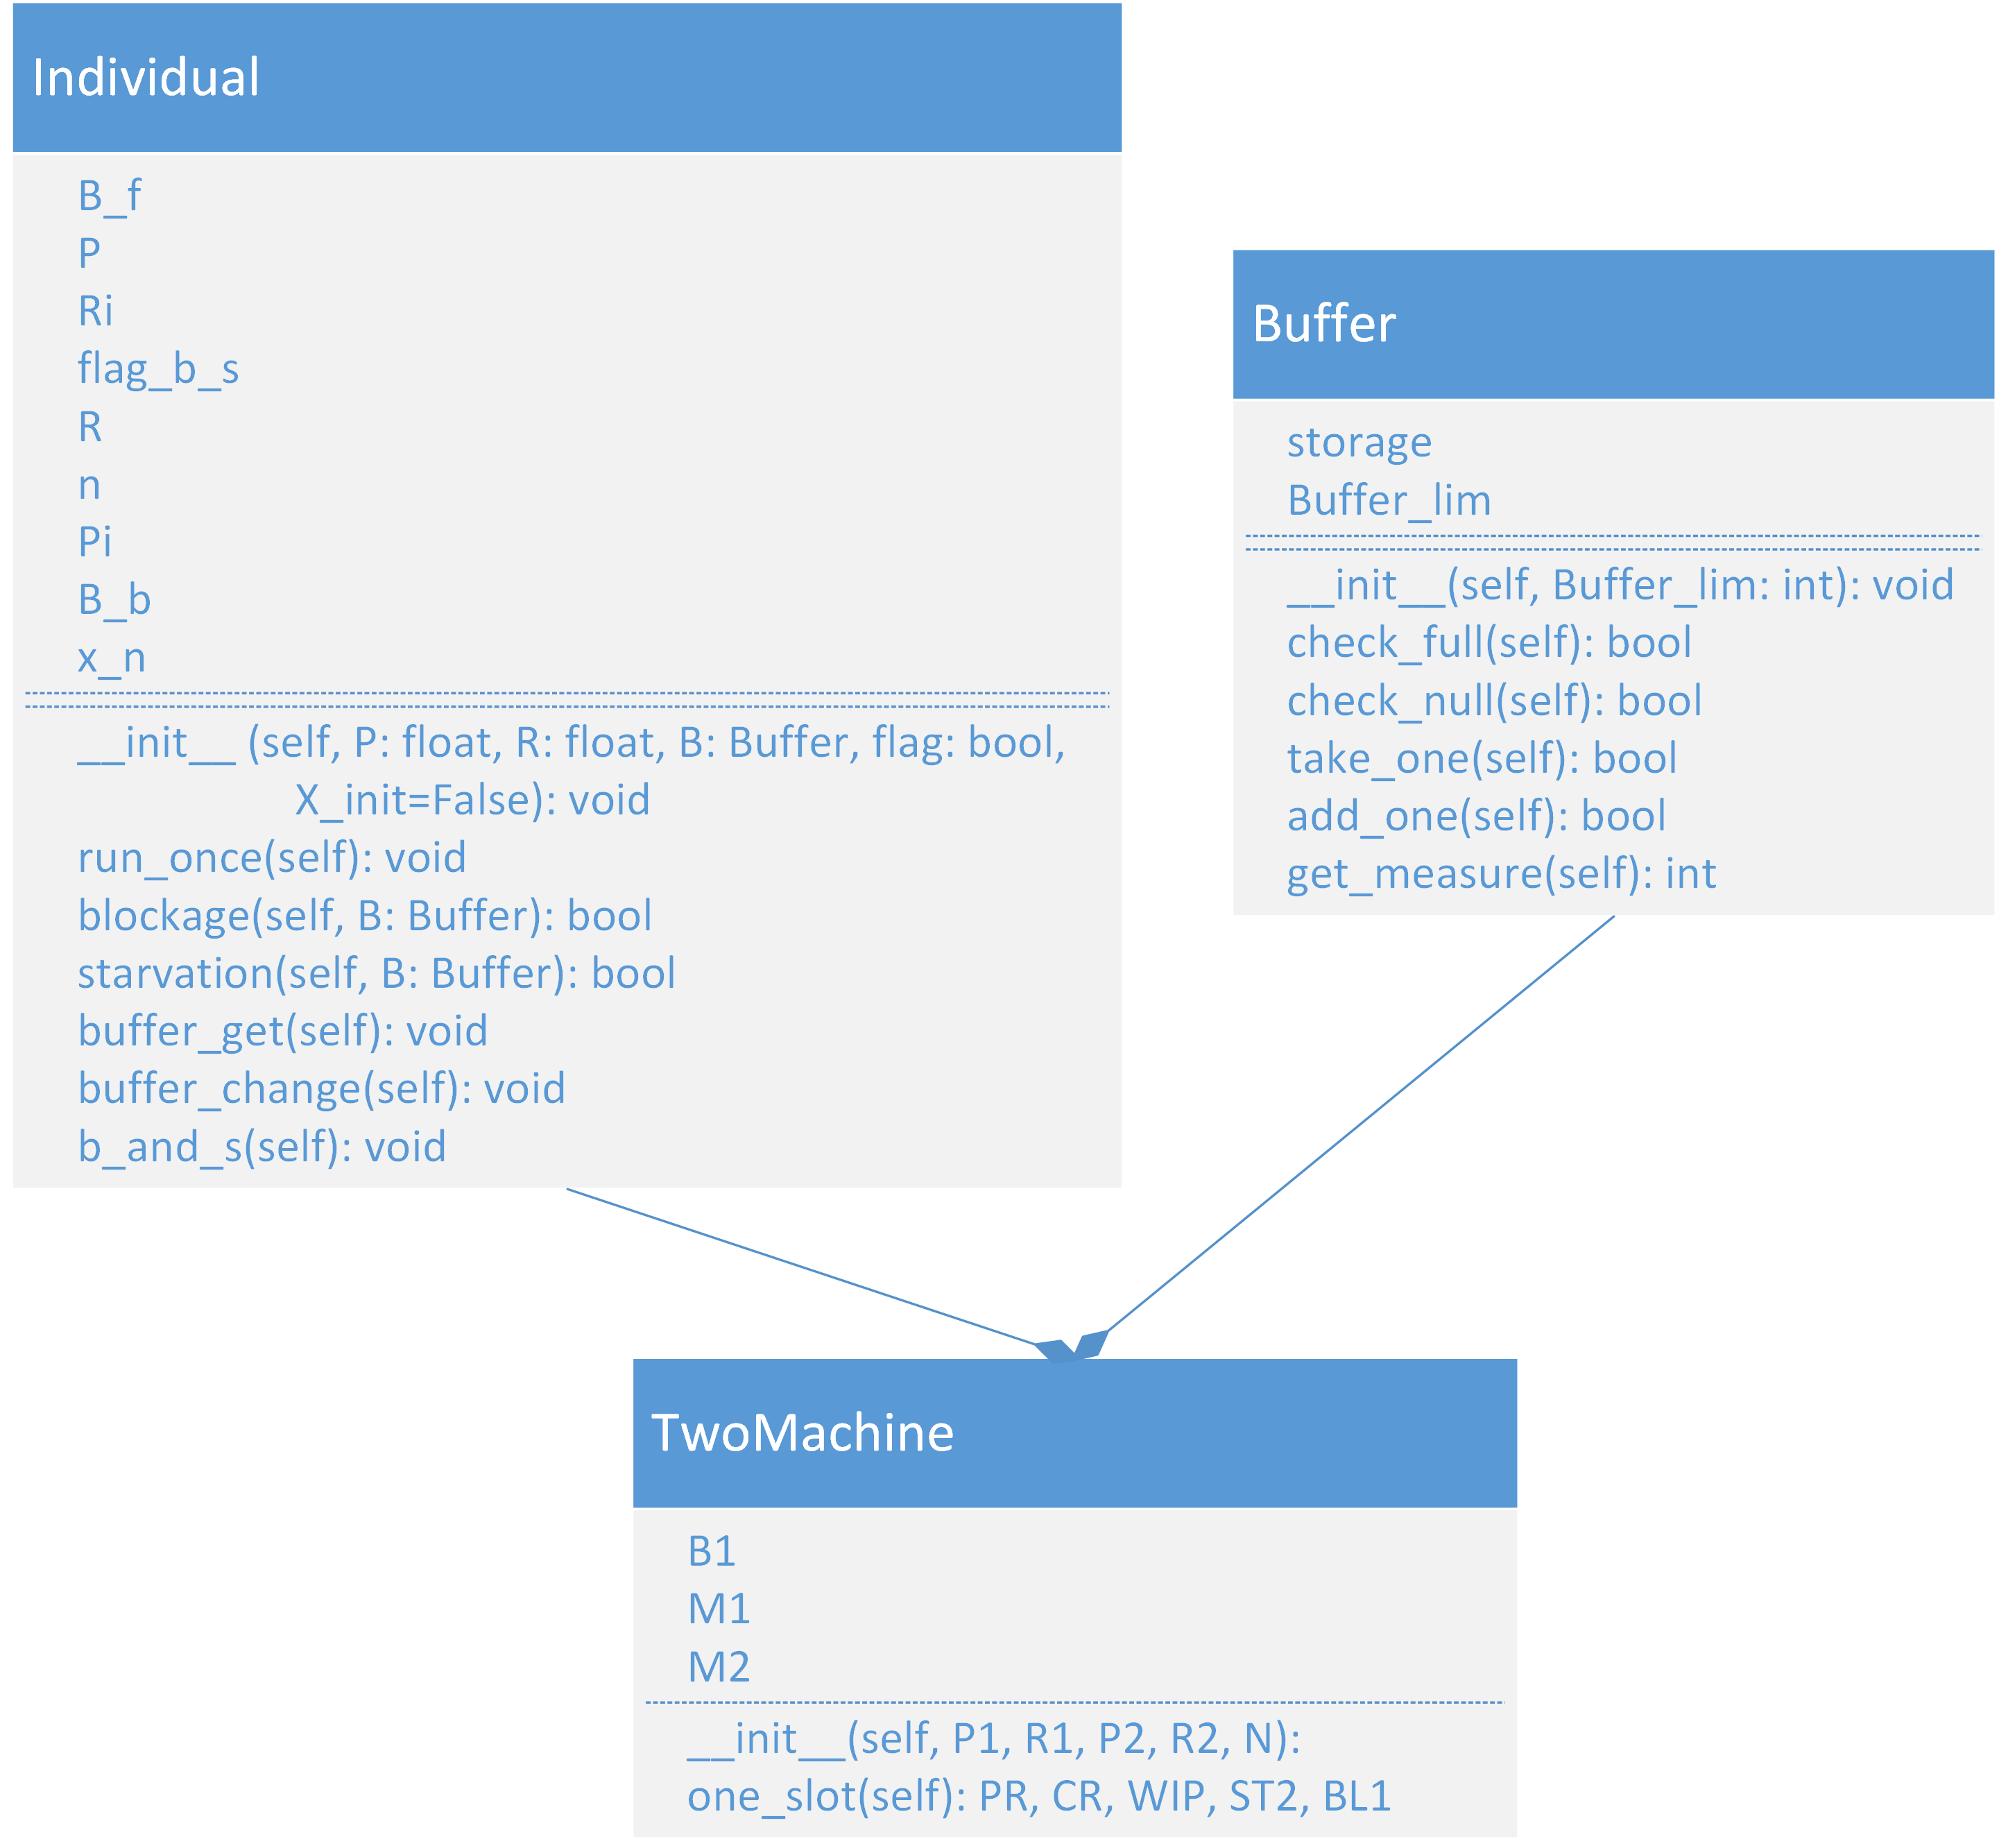
\includegraphics[width=0.8\linewidth]{two_machine.png}
	\caption{UML diagram of a two-machine model}
	\label{two machine uml}
\end{figure*}